\section{The HHL Algorithm}

\begin{figure}
    \centering
    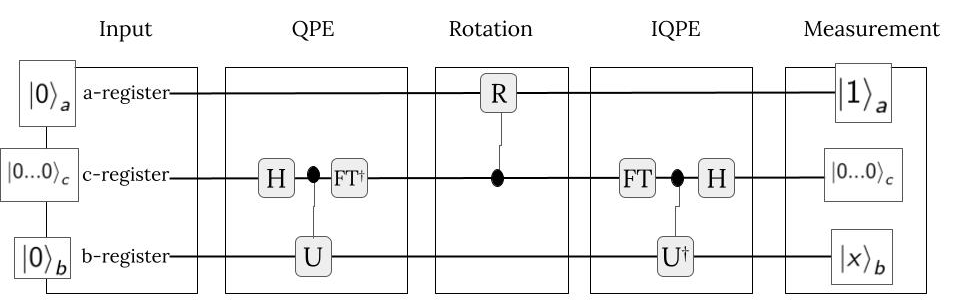
\includegraphics[width=8.5cm]{img/example_circuit_cropped.png}
    \caption{Example Circuit}
    \label{ex_circ}
\end{figure}

The next section will give a more detailed walkthrough of the HHL algorithm.
Thereby, it will go through all the 5 phases namely, state preperaration, QPE, inversion of eigenvalues, IQPE and lastly the measurement.

\subsection{State Preparation}

In total we have $n_b + n + 1$ qubits. 
In the beginning they are all initialized in their zero state as
\begin{equation}
\begin{split}
\ket{\Psi_0} &= \ket{0\dots0}_b\ \ket{0\dots0}_c\ \ket{0}_a \\
&= \ket{0}_b^{{\otimes n_b}}\ \ket{0}_c^{\otimes b}\ \ket{0}_a 
\end{split}
\end{equation}
We now have to load the vector $\vec{b}$ into the b-register. 
This is achieved by amplitude encoding. 

Todo 

insert formula here

The state $\ket b$ is then loaded into the b-register. Therefore

\begin{equation}
\ket{\Psi_1} = \ket{b}_b\ \ket{0\dots0}_c\ \ket{0}_a
\end{equation}

We have successfully encoded the $\vec{b}$ into our b-register. 
We now continue with the QPE. 

\subsection{Quantum Phase Estimation}
We will only briefly go through the specifics of the QPE and will not discuss each step in detail, as this is not the main topic of this paper. 
For further explanations refer to this paper.
As already mentioned, the QPE is a procedure to evalute an estimate of eigenvalues. 
It consists of three phases, namely the superpositions of the clock-bits via Hadamard gate, controlloed rotation via unitary U and the IQFT.
After QPE we will have an estimate of the eigenvalues of the unitary $U$. 
As we have encode $A$ as as a Hamiltonian $U = e^{iAt}$, the phase of the eigenvalue of U is proportional to the eigenvalue of $A$.
We have to define a scaled version of our eigenvalues $\lambda_j$.
\begin{equation}
\widetilde{\lambda_j} = \frac {N\lambda_jt}{2\pi}
\end{equation}
where t can be choosen freely so that $\widetilde{\lambda_j}$ are integers. 

Thus, the eigenvalues of $A$ will be stored in the c-register after QPE as
\begin{equation}
\begin{split}
\ket{\Psi_2} &= \ket{b}_b \ket{\widetilde{\lambda}}_c\ket{0}_a \\
% &=\left(-\frac{1}{\sqrt{2}} \ket{u_0} \ket{01} +\frac{1}{\sqrt{2}}  \ket{u_1} \ket{10} \right)  \ket{0}_a\\
& =\sum_{j=0}^{N-1} b_j \ket{u_j}_b \ket{\widetilde{\lambda}_j}_c \ket 0_a
\end{split}
\end{equation}
Notice, that the b-register is now a representation of the $\ket b$ state in the eigenbasis $\ket{u_j}$ of $A$.




